%!TEX root = ../thesis.tex

%%%%% Chapter: Tesseract OCR %%%%%
\chapter{Tesseract OCR}
\label{chap:tess-ocr}

\ifpdf
    \graphicspath{{Chapter4/Figs/Raster/}{Chapter4/Figs/PDF/}{Chapter4/Figs/}}
\else
    \graphicspath{{Chapter4/Figs/Vector/}{Chapter4/Figs/}}
\fi

\section{Overview}

In the system implementation, the Tesseract OCR engine is selected as the main tool which converts image data (handouts) to chunks of text. The Tesseract is able to do the Page Layout Analysis which identifies distinct chunks at 5 different scales. 

The Tesseract also provides a set of command-line tools which allow us to fine-tune the existing models. In order to improve the accuracy on handwritten text recognition, the original Tesseract model \texttt{eng} has been fine-tuned with additional handwritten data and evaluated at various training iterations. The best model has been picked based on the evaluation results.

\section{Multi-scale Page Layout Analysis}

Recall that the Page Layout Analysis of the Tesseract OCR engine is able to identify distinct blocks (or bounding-boxes) of text by analysing the general layout of the input document. The Tesseract engine can provide different sets of bounding boxes at 5 scales: word, line, paragraph, block and page.

\Cref{fig:tess-pla-scales} shows the Tesseract output bounding-boxes at 4 different scales, excluding the `page' scale since the output of the `page' scale just contains one bounding-box which is the image boundary.

\begin{figure}[!ht]
  \centering
  \begin{subfigure}{.42\textwidth}
    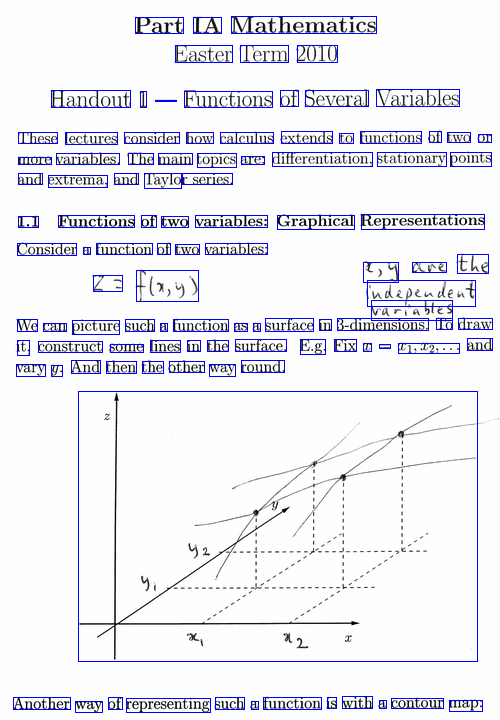
\includegraphics[width=\textwidth]{pla-word.png}
    \caption{Word scale}
  \end{subfigure}%
  \qquad
  \begin{subfigure}{.42\textwidth}
    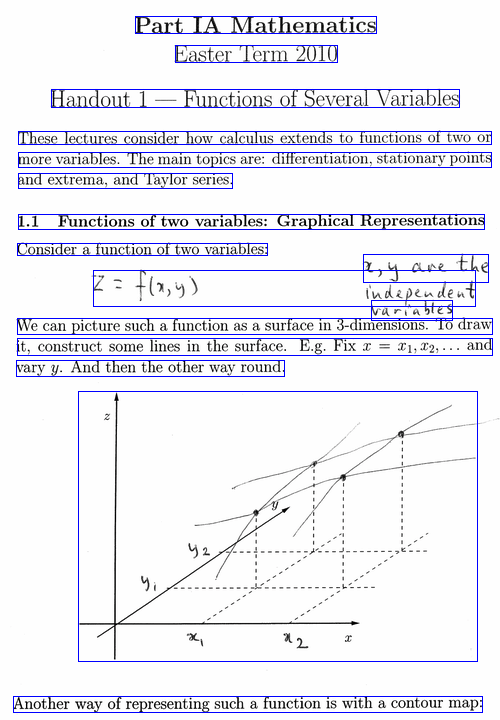
\includegraphics[width=\textwidth]{pla-line.png}
    \caption{Line scale}
  \end{subfigure}
  \vskip\baselineskip
  \begin{subfigure}{.42\textwidth}
    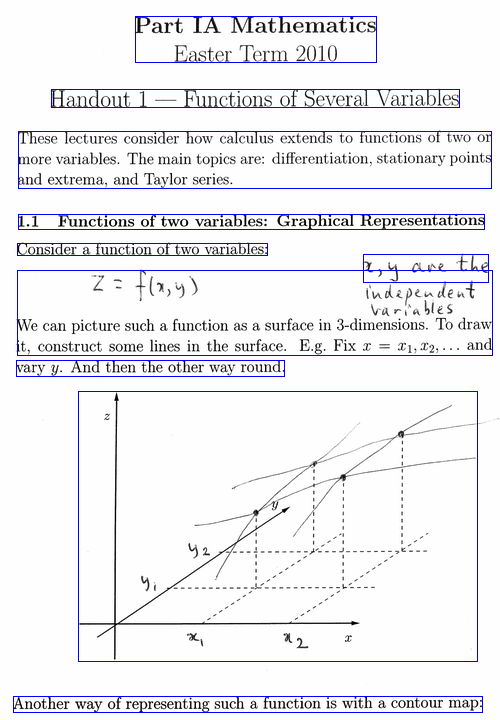
\includegraphics[width=\textwidth]{pla-par.png}
    \caption{Paragraph scale}
  \end{subfigure}%
  \qquad
  \begin{subfigure}{.42\textwidth}
    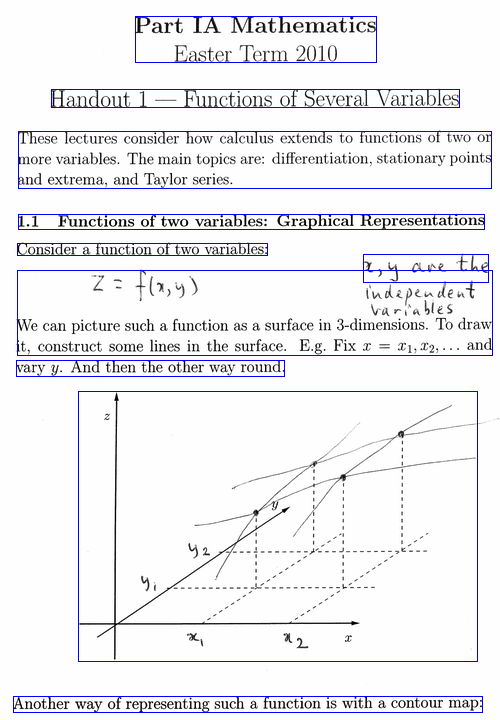
\includegraphics[width=\textwidth]{pla-block.png}
    \caption{Block scale}
  \end{subfigure}
  \caption{Different scales of Tesseract PLA}
  \label{fig:tess-pla-scales}
\end{figure}

In the actual system implementation, the user would be able to choose 4 different scales: word, line, paragraph and page. The `block' scale is removed from the implementation since in practice the difference between the `block' scale and the `paragraph' scale is negligible (which can be seen from \Cref{fig:tess-pla-scales}), and we keep the `paragraph' scale since the name `paragraph' is less ambiguous than `block'. 

The `page' scale actually remains in the system implementation for evaluation purposes, though this scale is not actually useful in practical use. The choice of PLA scale is considered to be one of the adjustable system parameters.

\section{Training Tesseract with Handwritten Data}

As mentioned in \Cref{sec:sys-arch-tess}, Tesseract allows us to fine-tune existing models to produce improved models, or retrain from scratch to make completely new models. In this project, we have fine-tuned the default English model using additional handwritten data, and have included the fine-tuned model in the system implementation. 

\subsection{Training Tools}

Since Tesseract itself is a command-line program, its training process also takes place in the command-lines. The original Tesseract training workflow requires extensive use of different commands with a large number of flags, which is very hard to handle in practice. Fortunately, there is a useful tool \cite{ocrd-train} which integrates all the required steps in the original training workflow in a Makefile. With this tool we only need to prepare the training data as images of textlines and simply run \texttt{make} in the terminal.

\subsection{Training Dataset}

In this project we have used the IAM Handwriting Database \cite{marti2002iam} as the training dataset. The IAM dataset is a collection of handwriting examples from 657 individual writers, and contains 13353 isolated and labelled text lines as PNG images and the corresponding label files. In the actual training, we use 95\% of the dataset for training and the rest 5\% is used for validation.

\subsection{Evaluation Dataset}

As we would like to see the actual performance of the fine-tuned model on our real handouts, a small dataset with 66 handwritten textlines extracted from Prof.\,Malcolm Smith's Part IA Mathematics handouts has been prepared for the model evaluation. 

Considering that when we fine-tune the Tesseract model with additional dataset, the model might forget its original parameters and thus perform worse in printed-text recognition compared to the original model. Therefore, we have also prepared another small dataset with 29 textlines of printed information from the same set of handout, in order to monitor the model performance on printed text during the training process.

\subsection{Performance vs Training Iterations}

\begin{figure}[!t]
  \centering
  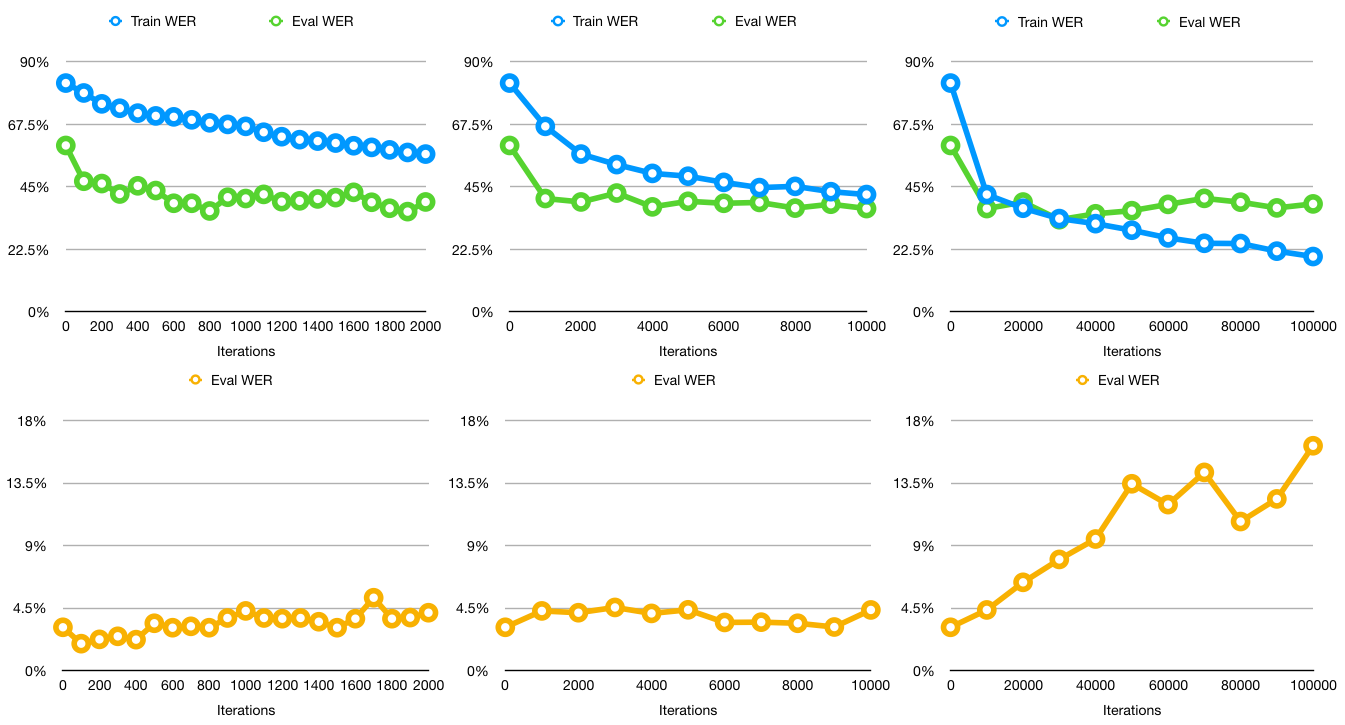
\includegraphics[width=.95\textwidth]{tess-eval.png}
  \caption{Training and Evaluation WERs on different datasets and iteration ranges}
  \label{fig:tess-eval}
\end{figure}

\Cref{fig:tess-eval} shows the plots of training and evaluation WERs at 3 iteration ranges: 0 - 2000 (first column), 0 - 10000 (second column) and 0 - 100000 (third column). The plots in the first row contain the training WERs on the IAM dataset and the evaluation WERs on the self-prepared small dataset of handwritten textlines, while the plots in the second row show the evaluation WERs on the self-prepared small dataset of printed textlines.

Base on the results in \Cref{fig:tess-eval}, we can see that the evaluation WER on the small handwritten dataset (green line) converges to around 45\% and the evaluation WER on the small printed-text dataset (yellow line) stays at around 4.5\% in the first 10000 iterations and starts to rise up after that. Since we aim to improve the recognition accuracy on handwritten text while not compromising the printed-text accuracy too much, we should limit our choices of model within the range of 10000 iterations.

\subsection{Selected Model}

Considering that the evaluation datasets are extremely small and the WERs are almost flat over the iteration range 0 - 10000, it is hard to make the decision and any choice within this range seems to be reasonable. Observing that there's a little dip in the yellow plot at iteration 9000, we have picked the fine-tuned model at iteration 9000 and have included this model as the alternative to the original Tesseract model.

Tesseract allows us to specify what model to use before running the OCR engine. The final system now contains two available models: the original one (named as \texttt{eng}) and the fine-tuned model at iteration 9000 (named as \texttt{eng-9000}). User can switch between the two models in the final software interface.